% Options for packages loaded elsewhere
\PassOptionsToPackage{unicode}{hyperref}
\PassOptionsToPackage{hyphens}{url}
\PassOptionsToPackage{dvipsnames,svgnames*,x11names*}{xcolor}
%
\documentclass[
]{krantz}
\usepackage{amsmath,amssymb}
\usepackage{lmodern}
\usepackage{ifxetex,ifluatex}
\ifnum 0\ifxetex 1\fi\ifluatex 1\fi=0 % if pdftex
  \usepackage[T1]{fontenc}
  \usepackage[utf8]{inputenc}
  \usepackage{textcomp} % provide euro and other symbols
\else % if luatex or xetex
  \usepackage{unicode-math}
  \defaultfontfeatures{Scale=MatchLowercase}
  \defaultfontfeatures[\rmfamily]{Ligatures=TeX,Scale=1}
\fi
% Use upquote if available, for straight quotes in verbatim environments
\IfFileExists{upquote.sty}{\usepackage{upquote}}{}
\IfFileExists{microtype.sty}{% use microtype if available
  \usepackage[]{microtype}
  \UseMicrotypeSet[protrusion]{basicmath} % disable protrusion for tt fonts
}{}
\makeatletter
\@ifundefined{KOMAClassName}{% if non-KOMA class
  \IfFileExists{parskip.sty}{%
    \usepackage{parskip}
  }{% else
    \setlength{\parindent}{0pt}
    \setlength{\parskip}{6pt plus 2pt minus 1pt}}
}{% if KOMA class
  \KOMAoptions{parskip=half}}
\makeatother
\usepackage{xcolor}
\IfFileExists{xurl.sty}{\usepackage{xurl}}{} % add URL line breaks if available
\IfFileExists{bookmark.sty}{\usepackage{bookmark}}{\usepackage{hyperref}}
\hypersetup{
  pdftitle={The back stories to publishing in Biological Sciences: a collection of reflections},
  pdfauthor={John Measey},
  colorlinks=true,
  linkcolor=Maroon,
  filecolor=Maroon,
  citecolor=Blue,
  urlcolor=Blue,
  pdfcreator={LaTeX via pandoc}}
\urlstyle{same} % disable monospaced font for URLs
\usepackage{color}
\usepackage{fancyvrb}
\newcommand{\VerbBar}{|}
\newcommand{\VERB}{\Verb[commandchars=\\\{\}]}
\DefineVerbatimEnvironment{Highlighting}{Verbatim}{commandchars=\\\{\}}
% Add ',fontsize=\small' for more characters per line
\usepackage{framed}
\definecolor{shadecolor}{RGB}{248,248,248}
\newenvironment{Shaded}{\begin{snugshade}}{\end{snugshade}}
\newcommand{\AlertTok}[1]{\textcolor[rgb]{0.33,0.33,0.33}{#1}}
\newcommand{\AnnotationTok}[1]{\textcolor[rgb]{0.37,0.37,0.37}{\textbf{\textit{#1}}}}
\newcommand{\AttributeTok}[1]{\textcolor[rgb]{0.61,0.61,0.61}{#1}}
\newcommand{\BaseNTok}[1]{\textcolor[rgb]{0.06,0.06,0.06}{#1}}
\newcommand{\BuiltInTok}[1]{#1}
\newcommand{\CharTok}[1]{\textcolor[rgb]{0.5,0.5,0.5}{#1}}
\newcommand{\CommentTok}[1]{\textcolor[rgb]{0.37,0.37,0.37}{\textit{#1}}}
\newcommand{\CommentVarTok}[1]{\textcolor[rgb]{0.37,0.37,0.37}{\textbf{\textit{#1}}}}
\newcommand{\ConstantTok}[1]{\textcolor[rgb]{0,0,0}{#1}}
\newcommand{\ControlFlowTok}[1]{\textcolor[rgb]{0.27,0.27,0.27}{\textbf{#1}}}
\newcommand{\DataTypeTok}[1]{\textcolor[rgb]{0.27,0.27,0.27}{#1}}
\newcommand{\DecValTok}[1]{\textcolor[rgb]{0.06,0.06,0.06}{#1}}
\newcommand{\DocumentationTok}[1]{\textcolor[rgb]{0.37,0.37,0.37}{\textbf{\textit{#1}}}}
\newcommand{\ErrorTok}[1]{\textcolor[rgb]{0.14,0.14,0.14}{\textbf{#1}}}
\newcommand{\ExtensionTok}[1]{#1}
\newcommand{\FloatTok}[1]{\textcolor[rgb]{0.06,0.06,0.06}{#1}}
\newcommand{\FunctionTok}[1]{\textcolor[rgb]{0,0,0}{#1}}
\newcommand{\ImportTok}[1]{#1}
\newcommand{\InformationTok}[1]{\textcolor[rgb]{0.37,0.37,0.37}{\textbf{\textit{#1}}}}
\newcommand{\KeywordTok}[1]{\textcolor[rgb]{0.27,0.27,0.27}{\textbf{#1}}}
\newcommand{\NormalTok}[1]{#1}
\newcommand{\OperatorTok}[1]{\textcolor[rgb]{0.43,0.43,0.43}{\textbf{#1}}}
\newcommand{\OtherTok}[1]{\textcolor[rgb]{0.37,0.37,0.37}{#1}}
\newcommand{\PreprocessorTok}[1]{\textcolor[rgb]{0.37,0.37,0.37}{\textit{#1}}}
\newcommand{\RegionMarkerTok}[1]{#1}
\newcommand{\SpecialCharTok}[1]{\textcolor[rgb]{0,0,0}{#1}}
\newcommand{\SpecialStringTok}[1]{\textcolor[rgb]{0.5,0.5,0.5}{#1}}
\newcommand{\StringTok}[1]{\textcolor[rgb]{0.5,0.5,0.5}{#1}}
\newcommand{\VariableTok}[1]{\textcolor[rgb]{0,0,0}{#1}}
\newcommand{\VerbatimStringTok}[1]{\textcolor[rgb]{0.5,0.5,0.5}{#1}}
\newcommand{\WarningTok}[1]{\textcolor[rgb]{0.37,0.37,0.37}{\textbf{\textit{#1}}}}
\usepackage{longtable,booktabs,array}
\usepackage{calc} % for calculating minipage widths
% Correct order of tables after \paragraph or \subparagraph
\usepackage{etoolbox}
\makeatletter
\patchcmd\longtable{\par}{\if@noskipsec\mbox{}\fi\par}{}{}
\makeatother
% Allow footnotes in longtable head/foot
\IfFileExists{footnotehyper.sty}{\usepackage{footnotehyper}}{\usepackage{footnote}}
\makesavenoteenv{longtable}
\usepackage{graphicx}
\makeatletter
\def\maxwidth{\ifdim\Gin@nat@width>\linewidth\linewidth\else\Gin@nat@width\fi}
\def\maxheight{\ifdim\Gin@nat@height>\textheight\textheight\else\Gin@nat@height\fi}
\makeatother
% Scale images if necessary, so that they will not overflow the page
% margins by default, and it is still possible to overwrite the defaults
% using explicit options in \includegraphics[width, height, ...]{}
\setkeys{Gin}{width=\maxwidth,height=\maxheight,keepaspectratio}
% Set default figure placement to htbp
\makeatletter
\def\fps@figure{htbp}
\makeatother
\setlength{\emergencystretch}{3em} % prevent overfull lines
\providecommand{\tightlist}{%
  \setlength{\itemsep}{0pt}\setlength{\parskip}{0pt}}
\setcounter{secnumdepth}{5}
\usepackage{booktabs}
\usepackage{longtable}
\usepackage[bf,singlelinecheck=off]{caption}
\usepackage[scale=.8]{sourcecodepro}

\usepackage{framed,color}
\definecolor{shadecolor}{RGB}{248,248,248}

\renewcommand{\textfraction}{0.05}
\renewcommand{\topfraction}{0.8}
\renewcommand{\bottomfraction}{0.8}
\renewcommand{\floatpagefraction}{0.75}

\renewenvironment{quote}{\begin{VF}}{\end{VF}}
\let\oldhref\href
\renewcommand{\href}[2]{#2\footnote{\url{#1}}}

\makeatletter
\newenvironment{kframe}{%
\medskip{}
\setlength{\fboxsep}{.8em}
 \def\at@end@of@kframe{}%
 \ifinner\ifhmode%
  \def\at@end@of@kframe{\end{minipage}}%
  \begin{minipage}{\columnwidth}%
 \fi\fi%
 \def\FrameCommand##1{\hskip\@totalleftmargin \hskip-\fboxsep
 \colorbox{shadecolor}{##1}\hskip-\fboxsep
     % There is no \\@totalrightmargin, so:
     \hskip-\linewidth \hskip-\@totalleftmargin \hskip\columnwidth}%
 \MakeFramed {\advance\hsize-\width
   \@totalleftmargin\z@ \linewidth\hsize
   \@setminipage}}%
 {\par\unskip\endMakeFramed%
 \at@end@of@kframe}
\makeatother

\renewenvironment{Shaded}{\begin{kframe}}{\end{kframe}}

\usepackage{makeidx}
\makeindex

\urlstyle{tt}

\usepackage{amsthm}
\makeatletter
\def\thm@space@setup{%
  \thm@preskip=8pt plus 2pt minus 4pt
  \thm@postskip=\thm@preskip
}
\makeatother

\frontmatter
\ifluatex
  \usepackage{selnolig}  % disable illegal ligatures
\fi
\usepackage[]{natbib}
\bibliographystyle{apalike}

\title{The back stories to publishing in Biological Sciences: a collection of reflections}
\author{John Measey}
\date{2021-08-22}

\begin{document}
\maketitle

% you may need to leave a few empty pages before the dedication page

%\cleardoublepage\newpage\thispagestyle{empty}\null
%\cleardoublepage\newpage\thispagestyle{empty}\null
%\cleardoublepage\newpage
\thispagestyle{empty}

\begin{center}
To Early Career Researchers who are struggling to publish...

we have all struggled to publish our work
%\includegraphics{images/dedication.pdf}
\end{center}

\setlength{\abovedisplayskip}{-5pt}
\setlength{\abovedisplayshortskip}{-5pt}

{
\hypersetup{linkcolor=}
\setcounter{tocdepth}{2}
\tableofcontents
}
\listoftables
\listoffigures
\hypertarget{welcome}{%
\chapter*{Welcome}\label{welcome}}


Sharing our successes and forgetting how we got there is not a true
reflection of the pains that many successful biologists go through when
publishing. The idea of this book is to openly share the struggle behind
the successes in many different published papers in the Biological
Sciences. In doing so, I hope that this book will represent a reflective
experience for those who author chapters about their work, in order to
look for the positive in what might otherwise be regarded as a
thoroughly negative experience. For those who read, this shared
community of practice should represent an insight into the failures that
everyone goes through - even though you might only see the success. In
addition, I hope that you can learn some tricks of our trade, in order
to better prepare you for your own publishing journey. Perhaps most
importantly, I want this book to provide some inspiration for those of
you who feel that you might want to give up. Publishing your work is
very important, we all want you to succeed, but sometimes you will need
to persevere in order to make the most of your research.

\hypertarget{requirements-for-contributors}{%
\chapter*{Requirements for contributors}\label{requirements-for-contributors}}


If you want to contribute to this book, there are a few requirements:

\begin{enumerate}
\def\labelenumi{\arabic{enumi}.}
\item
  You must have published the paper that your story is about, and
  provide a link to the paper, and if possible the online reviews
\item
  You should have been the principle author and/or certainly the
  corresponding author
\item
  This should have been an important paper for you personally, and
  preferably have some importance for others in your field. If it's
  not been a big deal for you, then it's not likely to make a good
  \textbf{back story}
\item
  Use the first person singular pronoun to tell your story
\item
  This is not an opportunity for \emph{ad hominem} attacks, so please avoid
  names of individuals
\item
  Make it personal about you and please do share your feelings. We
  want to know about the low times, but we also want to know what
  helped you through them
\item
  Use the exercise as an opportunity to reflect on your experience,
  and provide ideas that might help others who are faced with similar
  situation
\item
  Promote solutions. We know that the current world of publishing is
  not ideal. Provide some ideas for what you think might have worked
  in your situation
\end{enumerate}

\hypertarget{formula-for-contributors}{%
\chapter*{Formula for contributors}\label{formula-for-contributors}}


As long as you meet all of the \protect\hyperlink{requirements}{requirements} above,
there is no compulsory formula, and you are welcome to write your story
in your way. If you want some pointers of how you could structure your
chapter, then please see the outline below:

\begin{itemize}
\item
  Introduction: Tell us a little about you at the time that the study,
  and the write-up took place:

  \begin{itemize}
  \item
    what stage of your career were you at
  \item
    where in the world were you
  \item
    what was your home story at the time
  \item
    anything else that we need to know in order to appreciate your
    feelings and attachment to the study itself
  \end{itemize}
\item
  Back-story to the study: Briefly outline what the study was about:

  \begin{itemize}
  \item
    the approach \& ideas
  \item
    time taken to collect the data
  \item
    the other co-authors
  \item
    anything else relevant to understand the completion of the study
    and its write-up
  \end{itemize}
\item
  The first submission

  \begin{itemize}
  \item
    where did it go
  \item
    how long did it take
  \item
    what was the outcome
  \item
    what did you learn
  \end{itemize}
\item
  The second submission

  \begin{itemize}
  \tightlist
  \item
    see the first submission
  \end{itemize}
\item
  Repeat until accepted
\item
  Reflect on your experience:

  \begin{itemize}
  \item
    What were the major changes that you made to the manuscript
    between the first submission and acceptance
  \item
    Who made the difference between the rejections and acceptance of
    your paper and what did they do?
  \item
    What were the major lessons that you learned, and how has this
    changed your approach to publishing moving forwards?
  \item
    What advice can you give to Early Career Researchers who might
    be in the middle of their biggest publishing story, but not at
    the point where they have had their manuscript accepted?
  \end{itemize}
\item
  If you can, provide a picture or two that adds something personal to
  the story
\end{itemize}

\hypertarget{send-me-your-chapters}{%
\chapter*{Send me your chapters}\label{send-me-your-chapters}}


You can send chapters directly to me at
\url{john@measey.com}, or DM me on Twitter
\href{https://twitter.com/afriherp}{@AfriHerp}. This book will be published
\href{https://johnmeasey.github.io/How-to-publish-in-Biological-Sciences/openaccess1.html}{Open
Access}
online using \href{bookdown.org}{Bookdown} \citep{bookdown2016}. I will lightly
edit chapters prior to posting them. If you want to make it as easy as
possible, write your chapter in RMarkdown \citep{rmarkdown2018}, and please
send any citations in BibTex format.

If the book gets interesting, we can approach a publisher, but it should
always remain Open Access.

\hypertarget{software-information-and-conventions}{%
\section*{Software information and conventions}\label{software-information-and-conventions}}


I used the \textbf{knitr}\index{knitr} package \citep{xie2015} and the
\textbf{bookdown}\index{bookdown} package \citep{R-bookdown} to compile this book.
My R session information is shown below:

\begin{Shaded}
\begin{Highlighting}[]
\NormalTok{xfun}\SpecialCharTok{::}\FunctionTok{session\_info}\NormalTok{()}
\end{Highlighting}
\end{Shaded}

\begin{verbatim}
## R version 4.0.2 (2020-06-22)
## Platform: x86_64-w64-mingw32/x64 (64-bit)
## Running under: Windows 10 x64 (build 14393)
## 
## Locale:
##   LC_COLLATE=English_South Africa.1252 
##   LC_CTYPE=English_South Africa.1252   
##   LC_MONETARY=English_South Africa.1252
##   LC_NUMERIC=C                         
##   LC_TIME=English_South Africa.1252    
## 
## Package version:
##   base64enc_0.1.3   bookdown_0.21    
##   compiler_4.0.2    digest_0.6.25    
##   evaluate_0.14     glue_1.4.2       
##   graphics_4.0.2    grDevices_4.0.2  
##   highr_0.8         htmltools_0.5.1.1
##   jsonlite_1.7.2    knitr_1.31       
##   magrittr_2.0.1    markdown_1.1     
##   methods_4.0.2     mime_0.10        
##   rlang_0.4.10      rmarkdown_2.7    
##   rstudioapi_0.13   stats_4.0.2      
##   stringi_1.5.3     stringr_1.4.0    
##   tinytex_0.31      tools_4.0.2      
##   utils_4.0.2       xfun_0.20        
##   yaml_2.2.1
\end{verbatim}

\hypertarget{acknowledgments}{%
\section*{Acknowledgments}\label{acknowledgments}}


Thanks to everyone who has helped with the compilation of this book.

\begin{flushright}
John Measey\\
Cape Town
\end{flushright}

\hypertarget{about-the-editor}{%
\chapter*{About the Editor}\label{about-the-editor}}


John Measey is Associate Professor of Biological Sciences at Stellenbosch University. He has authored or co-authored more than \href{http://john.measey.com/Publications/Journal-Articles}{200 peer reviewed scientific papers} and \href{http://john.measey.com/Publications/Book-Chapters}{book chapters}, and \href{http://john.measey.com/Publications/Books}{six books}. He has been the Editor-in-Chief of an ISI journal for 9 years, and currently serves as Associate Editor for 4 other journals. He has graduated more than 20 postgraduate students, and his blog on writing and publishing in biological sciences is read by thousands globally. British born and educated, he lives and works in the beautiful Western Cape, South Africa.

\hypertarget{contribute}{%
\section*{Do you have something to contribute?}\label{contribute}}


This book is written in bookdown \citep{xie2016bookdown} specifically to make it a `live project' that will be open to anyone who wants to contribute, improve, or use as the basis for your own book. The easiest way for readers to contribute their own chapters as stories to to contact me (\url{john@measey.com}), or you can interact with the content directly through a \href{https://help.github.com/articles/about-pull-requests/}{GitHub pull request}. At the repository for this book, you will find Rmd files for each chapter, and as a GitHub user, you can simply edit the Rmd file and submit the changes. If I am happy with the changes proposed, I will merge your content with that of the book and add your name to the \protect\hyperlink{acknowledge}{Acknowledgements}.

One of the amazing potentials for \href{https://bookdown.org/}{bookdown books} is that all the files for this book are hosted in a repository on \href{https://github.com/johnmeasey/How-to-Publish-in-Biological-Sciences/tree/main}{Github}. You have the opportunity to fork this repository and write your own version for a different discipline, a different language or for a different region of the world. It is also my hope that this book can grow to become a community of practice for Early Career Researchers in Biological Sciences and other disciplines. This guide needs to be a `living document', and anyone who wants to provide feedback or contribute new sections is more than welcome. Please feel free to open an issue, or make a Pull Request if you spot a typo.

\mainmatter

\hypertarget{the-long-road-to-freshwater-paths}{%
\chapter{The long road to Freshwater Paths}\label{the-long-road-to-freshwater-paths}}

\textbf{John Measey}

\emph{Centre for Invasion Biology, Department of Botany and Zoology, Stellenbosch University, Stellenbosch, South Africa}

It all started when I read another paper written by a group of German researchers published in \emph{Proceedings of the Royal Society of London} \citep{vences2003multiple}. Their paper was exciting, they were using a phylogenetic approach to show that amphibians, without any doubt, had dispersed over marine barriers. I was fascinated, as at the time I had just come back from one such island with a set of endemic amphibian species. I settled down to read the paper and was enthused to see what they would say about my study site, and the amphibians it contained.

But the paper didn't mention them. In fact, before the end of the first paragraph of the introduction, it even denied that their existence:

\begin{quote}
``One important argument for such interpretations, ever since Darwin \citeyearpar{darwin1859origin}, has been that heretoforth no endemic amphibians were known from oceanic islands.''

\VA{---- \citet{vences2003multiple}}{}
\end{quote}

The rest of the study was very nice. They went on to explain how they could show that a group of amphibians had crossed an oceanographic barrier. But for me, I was stuck on that first paragraph and that they had completely overlooked my study site when I thought that everyone knew about it. After all, if I knew about it, then surely this group of distinguished German researchers should know?

It was 2003, and I was a Marie-Curie Fellow at Institut de Recherche pour le Développement (IRD) stationed at Bondy near Paris. I had already been there 18 months following a couple of short post-docs in South Africa and Brazil. But my fellowship wasn't going particularly well. I had visited the island of São Tomé on the recommendation of Bob Drewes (CalAcad), who I'd known for a number of years. Bob had spent nearly an entire conference banging on about São Tomé and how excellent it was, and how easy it was to find my study organisms: caecilian amphibians.



\begin{figure}
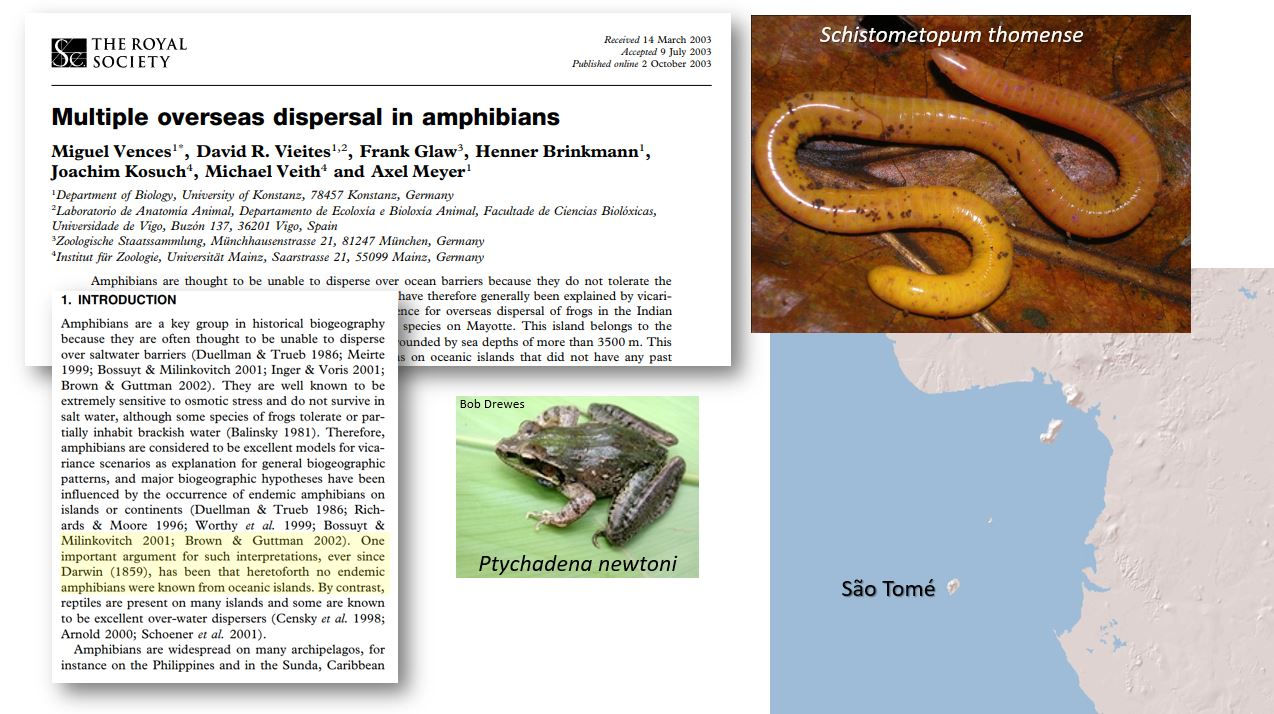
\includegraphics[width=0.85\linewidth]{figures/freshwater-paths} \caption{\textbf{A combination of events started the ball rolling on this manuscript}. The publication of \citet{vences2003multiple}, indoctrination from Bob Drewes about São Tomé, and my visits there in search of the `cobra bobo' (\emph{Schistometopum thomense}).}\label{fig:freshwater-paths}
\end{figure}

I emailed Bob, sent him a copy of Vences et al. \citeyearpar{vences2003multiple} and asked how it was possible that they had forgotten about São Tomé, and what were we going to do about setting the record straight. Bob fired straight back that we should contact Vences and ask why they hadn't included the (then) five known endemic species living on the island. Further, we asked whether Miguel would be interested in participating in a paper setting the record straight: that the endemic amphibians of São Tomé had undisputedly colonised the island by crossing a marine barrier, and that this had been (implicitly) known (although admittedly not explicitly stated) for more than 100 years \citep{bocage1873melanges}. São Tomé is one in a chain of volcanic islands (\textasciitilde13 Mya) in the Gulf of Guinea with minimum distances of at least 220 km from mainland Africa. The amphibians had been described since the mid-19th century, and their endemism had never been disputed. There followed some discussion and a delay while I went to Amsterdam to meet Miguel and sequence tissue that Bob had collected from an endemic frog (\emph{Ptychadena newtoni}) from São Tomé.

From this point on, what had been intended as a simple reply to Vences et al. \citeyearpar{vences2003multiple} became something far more complex and interesting. I had met oceanographers at IRD who worked in the Gulf of Guinea, and discussed ideas relating to the colonisation events of these islands. Bernad Bourles' data on oceanic currents and surface salinity was self-evident when put in this context. Lastly, Martim Melo was studying birds of the Cameroon line, and his expert knowledge about the island endemics was superlative - hence a comprehensive argument could be included about why the frogs had not been carried to the islands by birds.

\hypertarget{submitting-the-manuscript}{%
\section{Submitting the manuscript}\label{submitting-the-manuscript}}

The manuscript was finally finished and written up for \emph{Biology Letters} as it proposed a new explanation about how it was possible for amphibians to cross saltwater barriers using freshwater paths. I was proud of the paper, and I was sure that it was appropriate for \emph{Biology Letters}. It was submitted in September 2004, and it did get reviewed. One review was favourable, and the other pointed out four putative weaknesses, and suggested that for the paper to be more than conjecture some of these should be `strongly supported' in order make the paper convincing.

I appealed. I wrote a long explanation as to how in fact the manuscript already tackled three out of the four points convincingly, and that the fourth could at least be given a high probability. I have no record of whether or not the appeal was even considered. Presumably not. So I was resigned to picking out another journal. Discussion ensued, and we decided on \emph{Journal of Biogeography}. This required re-writing the manuscript as a full paper, but on reflection this also allowed me to pull in a lot more of my reading into the manuscript and more convincingly address the points raised by Reviewer \#2 from our \emph{Biology Letters} submission.

The new manuscript was submitted to \emph{Journal of Biogeography} early in 2005, and once again it was reviewed. The reviews took a long time. I think I must have written and asked about it as the decision email started with an apology. This time the reviewers were not short and punchy, but very long, asking for a substantial rewrite, and more sequencing of the specimens to produce a more convincing phylogeny. My fellowship had ended and I was unemployed. Still working on manuscripts as well as funding applications, job applications and all those other occupations that make the life of an unemployed Early Career Researcher so much more painful and unfulfilling than those in work. Discussions about the reviews ensued, and it was decided that we needed to do the additional sequencing to produce the new phylogeny, and that this could be done by a new postgraduate of Miguel's, Ylenia Chiari, while I got to work rewriting and responding to the text.

This was a real low point for me. I had a crisis in confidence as I was an inexperienced researcher trying to head up an important paper with much more senior scientists and fellow ECRs as co-authors. What did they think of how I was handling the manuscript? Had I imagined the importance of this work? Should I rather hand the manuscript over to someone with more experience? At the same time, the slow progress on this manuscript was impeding momentum on my career. I really wanted to be able to have this as a completed project. Lastly, I had that nagging doubt that someone, maybe even the reviewers, would publish on this subject before me. Many people had now seen this idea, and they all had access to similar resources that could provide similar lines of evidence. It was an uncomfortable time during which I came to believe that the manuscript would never be published.

That hiatus of doubt, sequencing and rewriting might have lasted as long as a year to 18 months. At long last, the sequencing and reanalysis was done and the manuscript rewritten with the extensive reviewer comments addressed.

the manuscript was again ready to submit and send back to \emph{Journal of Biogeography.} More time passed. This time we managed to get a decision of Minor Revision, but the reviewers wanted us to change the title of the manuscript. They didn't like ``Freshwater Paths'' and I felt heartbroken because this was at the crux of the manuscript, the idea that enough freshwater was exiting the Congo River in a very large plume that would lower sea-surface salinity all the way to the Gulf of Guinea islands. Under duress, I changed the title.

Happily for me, the \emph{Journal of Biogeography} handling editor was Bob McDowell. Bob liked the title and urged me to change it back again. He also had quite a lot of suggestions to improve the readability of the text. Suddenly, I felt as if I was turning the corner on this manuscript. An editor liked it and was prepared to make sure that it was as good as it could be before going to print. It did shuttle forwards and backwards again a few times between myself and the \emph{Journal of Biogeography} editorial team, but by then I had the feeling that it would all come out ok. Things were also looking up for me as I had a new postdoc starting. The paper was published in 2007: Measey et al. \citeyearpar{measey2007freshwater}.



\begin{figure}
\includegraphics[width=0.85\linewidth]{figures/Dscn4787} \caption{\textbf{Time spent on São Tomé also had its ups and downs}. My field assistant Quintino Quade celebrates our fantastic haul of caeclians, after a day spent digging in the rain in the island's forested interior.}\label{fig:celebrate}
\end{figure}

\hypertarget{looking-back}{%
\section{Looking back}\label{looking-back}}

At the time, I would have been happy had the manuscript been accepted in \emph{Biology Letters}, but it would not have been nearly as good as the manuscript that was accepted at the \emph{Journal of Biogeography.} The reviewers that I was convinced were trying to make life as difficult as possible for the manuscript, had made it a lot better. I think that the editors of the \emph{Journal of Biogeography} had made a huge difference in their commitment to getting a good manuscript for their journal.

The payoff has been that this has been one of my best cited papers over the years, and it's a publication that I'm proud of. It introduced me to a better way of collaboration over antagonism when responding to an error made by colleagues, and it resulted in lots of connections with people from other disciplines that I would not have otherwise met.

The study has inspired others too. I've had a bunch of different undergraduates telling me that they read the paper as a part of their course, and enjoyed it (something that doesn't happen too often). In addition, the study became the subject of a chapter in a popular book about biogeography by Alan de Queroz \citeyearpar{dequeiroz2014monkey}: \href{https://monkeysvoyage.wordpress.com/}{The Monkey's Voyage}: How Improbable Journeys Shaped the History of Life.

\hypertarget{doing-things-the-old-way}{%
\chapter{Doing things the old way}\label{doing-things-the-old-way}}

\textbf{Brian van Wilgen}

\emph{Centre for Invasion Biology, Department of Botany and Zoology, Stellenbosch University, Stellenbosch, South Africa}

Back in the late 1970s, I was an MSc student working on a thesis about the effects of fire in fynbos vegetation; a biodiverse heathland vegetation endemic to South Africa's southwestern region. I was employed by the Department of Forestry, and based at the Jonkershoek Forestry Research Centre near Stellenbosch, South Africa. It was a time when the Department was about to embark on an ambitious program to introduce prescribed burning to vast areas of mountain fynbos, and they needed scientific studies to provide a basis for knowing how often, and when, to burn. It was an exciting period to be a researcher in this field, because at that time the entire collection of scientific papers about the ecology of fynbos could be stored in a single small folder. It was also conventional to write a thesis as a single, stand-alone document, but universities were beginning to experiment with the idea of preparing each chapter as a paper that could be submitted to a journal for publication. Consequently, I was advised to follow this route.

My study examined the effects of frequency of burning on fynbos vegetation. I used three sites to compare outcomes -- one that was burnt every four years, one that burnt every 20 years or so, and one that had been protected from fire for 37 years. I had two potentially publishable papers in my thesis, one that dealt with the botanical composition of the sites, and one with the above-ground biomass. My research confirmed that burning at four-year intervals eliminated tall proteas (family Proteaceae), reducing the vegetation to a short stature with low biomass. Burning every 20 years resulted in stands of healthy proteas, with much more above-ground biomass. Protection from fire for longer periods resulted in the proteas becoming senescent, with excessive amounts of dead, dry material above ground. At the time, it was policy that all research done in the department had to be published in the \emph{South African Forestry Journal}, which was not rigorously peer-reviewed. My academic supervisor, Dr Eugene Moll at UCT, thought that the biomass paper would be suitable for an international journal, and encouraged me to submit it to the \emph{Journal of Ecology}. This break with protocol required lengthy negotiations with the department, but in the end they allowed me to submit the paper to the journal.



\begin{figure}
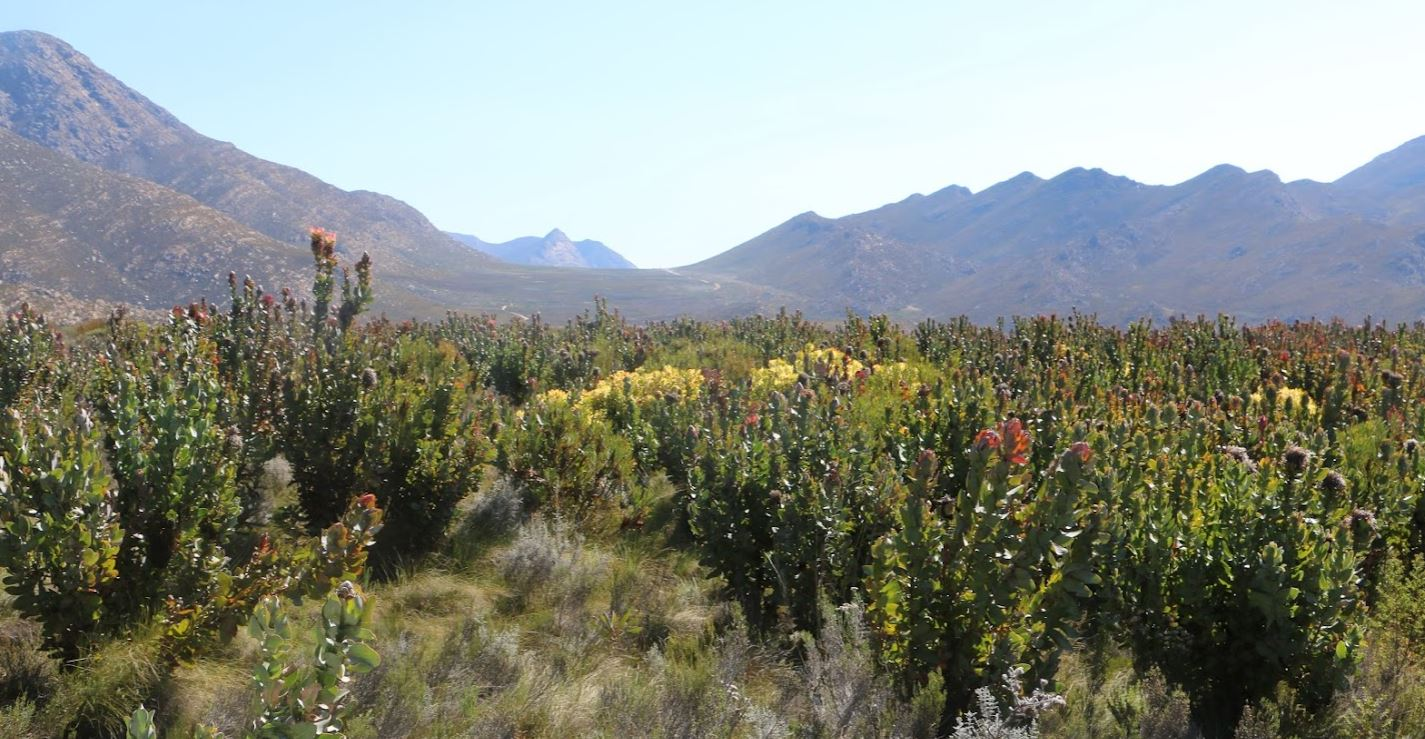
\includegraphics[width=0.95\linewidth]{figures/proteas-in-fynbos} \caption{\textbf{Proteas growing in the fynbos}. The fynbos is a fire dependent vegetation, but if fires don't burn frequently enough, proteas like these become tall and woody.}\label{fig:proteas-in-fynbos}
\end{figure}

\hypertarget{submitting-the-manuscript-1}{%
\section{Submitting the manuscript}\label{submitting-the-manuscript-1}}

Things were very different in those days. Everything was done on hard copies, and we used the postal service to submit and receive documents. Receipt was acknowledged with postcards. Manuscripts were prepared with a device called a typewriter, and figures had to be prepared by hand using graphic artists and manufactured sheets of typefaces and other elements (e.g.~\href{https://en.wikipedia.org/wiki/Letraset}{Letraset}) that were transferred manually to the artwork. Once my manuscript on the effects of fire frequency on fynbos biomass was ready, I placed it (and three additional copies to be posted on to reviewers) all into an envelope, stuck stamps on it, and posted it off to England. If I could have held my breath and kept my fingers crossed for the next three months, I would have done so.

Eventually, a large manilla envelope, festooned with British stamps and addressed to ``Doctor'' BW van Wilgen appeared in my postbox. In it was a covering letter from the editor handling the manuscript, who said that the journal may be interested in publishing the paper, provided that rather a lot of changes were made to bring the paper up to a standard that they would be happy with. Accompanying this was a copy of the manuscript with corrections indicated in pen. Some words were crossed out, others were added, and words or parts of sentences were ringed, with arrows showing where they should be moved to new positions. When I looked at this, I could see that the editor obviously knew their stuff, and that they had done one heck of a lot to improve my grammar, syntax and logic. I very carefully attended to all of this, prepared a new manuscript, and posted it back to England.

This time, only two months passed before another envelope arrived in my postbox. It was another painstakingly marked-up version of my manuscript, with a cover letter expressing appreciation for my clumsy attempts to improve the paper, and requesting a further round of corrections. I worked through all of this again, and prepared a marked-up version for the typist to attend to. The typist indicated that it would have to go into the queue of other work, and that they would not be able to realistically get to it before the end of next week. I was appalled at this delay. I then, somewhat foolishly, decided to re-type the manuscript myself to speed things up. This was a painstaking process, as I had no training. I had to search for each letter on the keyboard before hitting the lever that imprinted the letter onto the paper. I used the two index fingers on both hands to do this, which made me look like a chicken pecking at seeds on the ground (it is a technique I use to this day, much to the amusement of my colleagues, but I am a little faster now). Of course, any mistake you made meant that you had to start the whole page over again. Needless to say, the typist cleared their backlog before I was halfway done, and rapidly completed the job for me.

Another round of review followed, and this time the manuscript was returned requiring further, but much less extensive, changes. These I attended to, and received by return of post a letter saying that the handling editor was happy with the paper, and would now pass it on to the Editor-in-Chief for a final decision. To my dismay, another marked-up version appeared in my post box about a month later. Further edits were required. The editor also wanted the title of the article to change from ``effects of fire frequency'' to ``effects of post-fire age'', saying that it was with consternation that he noted that this rather fundamental point had not yet been picked up. He also told me to remove a figure, in which I had drawn curved lines through three data points showing how live biomass first increased, and then decreased, with increasing post-fire age, while at the same time the mass of dead material increased at first gradually, the exponentially. He told me that my carefully-prepared figure ``owed more to art than to science'', so I replaced it with a description. After this, my paper was accepted in the \emph{Journal of Ecology}, and finally appeared in print one and a half years after the first submission: van Wilgen \citep{vanwilgen1982effects}.



\begin{figure}
\includegraphics[width=0.85\linewidth]{figures/BvW-plot} \caption{\textbf{Brian van Wilgen collecting plot data in the fynbos, 1978}. This recently burned plot of fynbos is dominated by proteas (front left) that are all very small.}\label{fig:BvW-plot}
\end{figure}

\hypertarget{looking-back-1}{%
\section{Looking back}\label{looking-back-1}}

I was immensely proud of this paper. I had managed to get published in a leading international journal, and I was on my way to becoming a real scientist. This was thanks in no small part to some quality editing on the part of the journal, something that is not always the case today. More importantly, the process had taught me lessons that have stood me in good stead ever since. These included the importance of saying what was necessary in as few words as possible, and how to structure a logical progression from introduction, through methods and results to discussion. Most of all, it taught me the importance of attention to detail. Researchers in the 21st century have constant access to word processors, graphics packages for preparing figures, statistical packages for analyzing data, and online access to published papers. While all of this has made it so much easier to write and produce papers, it also makes it easy to cut corners and sometimes to become sloppy. When you can simply add, delete or move a sentence without having to retype the whole page (or add a paragraph without having to retype the rest of the manuscript), you could inadvertently make things worse. My advice would always be to spend additional time getting things as close to perfect the first time around. It will increase the chances of your paper getting a positive reception, and in the long run save time in the revision stages.

\hypertarget{the-next-chapter}{%
\chapter{The Next Chapter}\label{the-next-chapter}}

Your story could go next\ldots{}

\cleardoublepage

\hypertarget{appendix-appendix}{%
\appendix \addcontentsline{toc}{chapter}{\appendixname}}


\hypertarget{the-final-word}{%
\chapter{The final word}\label{the-final-word}}

Thanks to everyone who has contributed to this book so far. It's great to share and reflect on our journeys, and I know that I've enjoyed looking back on my own publishing story.

I had this idea when I was out on a run. I'm constantly amazed that running time is so productive in terms of generating ideas, rethinking plans and experiments. I love my running space. It's inspirational on so many levels. Here's a snap I took from the highest point:

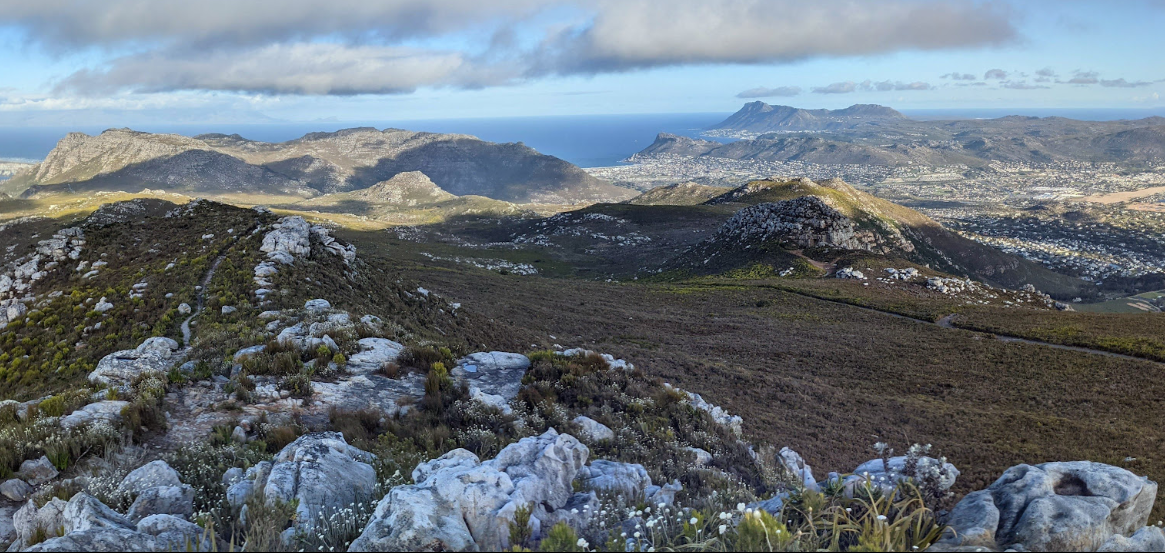
\includegraphics{figures/running-space.PNG}

By this point in the run (17:00 on 19 August 2021), I'd had the idea and decided to go home and get it ready for people to contribute. From this point, it's mostly downhill. If you ever feel that you need some inspiration, I urge you to get out into your world and move as you think.

To see more \textbf{bookdown} books, go to \url{https://bookdown.org}.

  \bibliography{book.bib,packages.bib}

\backmatter
\printindex

\end{document}
